%===========[ PREAMBLE ]========================================================
\documentclass[11pt]{article}
\usepackage[utf8]{inputenc}
\usepackage[english]{babel}
\usepackage[a4paper, top=0.98in, bottom=0.79in, left=0.98in, right=0.98in]{geometry}
\usepackage{graphicx}
\usepackage{tabularx}
\usepackage{fancyhdr}
\usepackage{setspace}
\usepackage{titlesec}
\usepackage{enumitem}
\usepackage{todonotes}
\usepackage{csquotes}
\usepackage{listings}
\lstset{language=SPARQL,breaklines=true}
\usepackage{siunitx}
\usepackage[labelsep=period]{caption}
\usepackage{mwe}
\usepackage{xfrac}
\usepackage[colorlinks=true,urlcolor=blue]{hyperref}
\usepackage{cleveref}
\usepackage{aurl}
\daurl{bb}{http://www.snik.eu/ontology/bb/}
\daurl{ob}{http://www.snik.eu/ontology/bb/}
\daurl{meta}{http://www.snik.eu/ontology/meta/}
\graphicspath{{./img/}}
\usepackage[backend=biber, style=ieee]{biblatex} %For bibliography management with biblatex
\addbibresource{paper.bib}
\addbibresource{snik.bib}
\addbibresource{relatedwork.bib}

% ==========[ FONT ]============================================================
%For the font of the document uncoment one of the following options.
%If using pdflatex compiler the follwoing commands will provide an arial-like
%font (helvetica)
\usepackage{helvet}
\renewcommand{\familydefault}{\sfdefault}
%If using xelatex compiler the follwoing commands will provide arial font
%\usepackage{fontspec}
%\setmainfont{Arial}

%===========[ FORMAT ]==========================================================
%Please do not edit or remove these lines
\pagenumbering{gobble}
\setlength{\parskip}{6pt}
\setlist[1]{topsep=0pt,itemsep=-5pt}
\addto\captionsenglish{\renewcommand{\figurename}{Figure}}
\addto\captionsenglish{\renewcommand{\tablename}{Table}}
\titlespacing*{\section}{0pt}{10pt}{4pt}
\titlespacing*{\subsection}{0pt}{0ex}{0pt}
\titlespacing*{\subsubsection}{0pt}{0pt}{0pt}
\titlespacing*{\paragraph}{0pt}{6pt}{6pt}
\captionsetup{belowskip=0pt,skip=6pt,labelfont=bf}%justification=raggedright,singlelinecheck=false
\makeatletter
\renewcommand{\maketitle}{
    \begin{flushleft}
        \footnotesize{Placeholder Name of the conference}\\\medskip
        \footnotesize{Placeholder Session title}\\\medskip
        \footnotesize{https://doi.or/10........ DOI placeholder (WILL BE FILLED IN BY TIB Open Publishing)}\\\medskip
        \footnotesize{\textcopyright\ Authors. This work is licensed under a \href{https://creativecommons.org/licenses/by/4.0/}{Creative Commons Attribution 4.0 International License}}\\\medskip
        \footnotesize{Published: (WILL BE FILLED IN BY TIB Open Publishing)}\\
    \end{flushleft}
    \begin{center}
        \LARGE\textbf{\contribtitle}\\\smallskip
        \Large{\contribsubtitle}
    \end{center}
    \normalsize{\firstauthor, \secondauthor, and \thirdauthor}
    \begin{center}
        \textsuperscript{1}\footnotesize{\firstauthoruniv}\\\medskip
        \textsuperscript{2}\footnotesize{\secondauthoruniv}\\\medskip
        \textsuperscript{3}\footnotesize{\thirdauthoruniv}\\\medskip
    \end{center}}
\makeatother

%===========[ TITLES ]==========================================================
%Chnage to your own information
%\newcommand{\contribtitle}{FAIR Knowledge Graphs for the Management of Health Information Systems}
\newcommand{\contribtitle}{SNIK Graph}
\newcommand{\contribsubtitle}{Visualizing Knowledge about Management of Hospital Information Systems}
%\newcommand{\contribsubtitle}{Graph-Based Exploration of an Hospital Information Systems}
\newcommand{\firstauthor}{Konrad Höffner\textsuperscript{1[https://orcid.org/0000-0001-7358-3217]}}
\newcommand{\firstauthoruniv}{Institute for Medical Informatics, Statistics and Epidemiology (IMISE), Germany}
\newcommand{\secondauthor}{Thomas Pause\textsuperscript{2[https://orcid.org/0000-0001-5832-4890]}}
\newcommand{\secondauthoruniv}{Institute for Medical Informatics, Statistics and Epidemiology (IMISE), Germany}
\newcommand{\thirdauthor}{Franziska Jahn\textsuperscript{3[https://orcid.org/0000-0002-7687-8544]}}%\todo{fj: orcid bitte anpassen}
\newcommand{\thirdauthoruniv}{Institute for Medical Informatics, Statistics and Epidemiology (IMISE), Germany}

%===========[ CONTENT ]=========================================================
\begin{document}
\maketitle

\paragraph{Abstract.}% The abstract should summarize the contents of the paper in short terms, i.e. in up to 250 words.
% ~ 150 words
Medical and health informatics integrates knowledge of business information systems, computer science and medicine.
As a comparatively young research discipline, it lacks a uniform terminology, especially for describing health information systems and their management.
SNIK, the semantic network of information management in hospitals, is an ontology that combines the knowledge of three textbooks, the IT4IT standard and an interview with a hospital CIO.
Graph-based visualizations allow teachers to intuitively convey relationships between a selection of those concepts and also allow students to explore the domain on their own.
We present SNIK Graph, a web-based client-side open-source Linked Data visualization for both classes and instances that is optimized for teaching and studying knowledge about the management of health information systems.
Due to the large amount of concepts and relationships, visualizing SNIK as a graph causes overplotting, which we solve using filters, searches and exploratory operations. 
%Students of medical informatics need to internalize complex relations between large amounts of concepts of health information systems (HIS) and their management.
%We present SNIK Graph, a graph-based linked data visualization web application that supports teaching textbook knowledge about HIS management.
\paragraph{Keywords:} Linked open data visualization, health information systems, information management, 

\section*{Introduction}%
Medical and health informatics integrates knowledge of business information systems, computer science and medicine.
As a comparatively young research discipline, it lacks a uniform terminology, especially for describing health information systems and their management.
Several textbooks provide different perspectives of the discipline but the linear struture inherent in a book does not intuitively convey the highly connected nature of the concepts of the domain.
Thus, preparing students for practical or scientific work in the domain of health information systems requires an integrated system of concepts linking the terms of the different disciplines.
SNIK, the semantic network of information management in hospitals, is an ontology linking the knowledge of three textbooks~\cite{bb,ob,he}, the IT4IT standard~\cite{it4it}, and a CIO's knowledge about information management at a certain German university hospital.
It thus integrates theoretical knowledge of medical informatics and information systems as well as practical knowledge from industry and a health institutions.
%The SNIK ontology is visualized by SNIK Graph.

Graph-based visualizations allow teachers to intuitively convey relationships between a selection of those concepts and also allow students to explore the domain on their own~\cite{ontologybased}.
There are several existing graph-based Linked Data visualizations~\cite{linkeddatavisualization}, which visualize RDF resources (classes or instanes) as nodes and their relationships as edges.
but they do not fit our requirements~\cite{visualizationoflargeontologies}.
Our contribution is SNIK Graph, a web application\footnote{\url{http://www.snik.eu/graph}} that offers Linked Data visualization for both classes and instances and according to the requirements of SNIK and its users.
%The graph is visualized using the Cytoscape.js~\cite{cytoscapejs} library with the force-directed Euler layout. %, see%~\cref{fig:snik-graph-overview}.
With the thousands of classes of SNIK, graph-based visualization suffers from overplotting.
Thus, SNIK Graph offers several options to select and layout subgraphs, for example to show only a specific chapter of a book to prepare a lecture about a specific topic.
Users can also iteratively explore SNIK starting at a single class using neighbourhood and path operations. %(see \cref{fig:snik-graph-circle-star})
% and subsequently the neighbourhood of selected neighbours of the previous step.
%SNIK Graph can also calculate the shortest path to between classes.
%Path and neighourhood operations are joined in the \enquote{spider worm}
%(see \cref{fig:snik-graph-spiderworm})
%, which consists of the shortest path between a start node and an end node together with the end node’s neighbourhood, illustrate the context of a concept.


%\subsection*{Motivation}%
%They also allow students of medical informatics internalize complex relations between large amounts of concepts of health information systems and their management~\cite{visualizationoflargeontologies}.
%\cite{snikgraphposter}
%
%A large amount of relevant knowledge is freely available as Linked Open Data.
%This structured approach is well suited for consumption by machines but basic access mechanisms like the text-based RDF serializations and SPARQL queries are not well suited for humans for large knowledge bases, especially for non-expert users.
%While the Semantic Web field has been providing a wealth of knowledge and is increasingly adopted by mainstream industries, not all use cases are yet supported by easy-to-use tools~\cite{semanticwebfield}.
%One such use case is graph-based exploration, where RDF data is displayed as a directed graph, with the resources as nodes and the triples as edges.
%As existing approaches \iffalse(see \cref{sec:relatedwork})\fi do not satisfy the needs of the students and researchers for exploring Hospital Information Management as Linked Open Data in the SNIK ontology~\cite{sniktec}, we implement \emph{SNIK Graph} as an easy-to-use graph-based web application, which we present in the following.
%To minimize duplicated 
%One such area is exploration, where users intuitively 
%Easy-to-use and freely available tools exist for 
%However, there is a lack of easy-to-use tools along the whole lifecycle of data~\cite{semanticwebfield}.
% - software is hard to publish
%The SNIK ontology~\cite{sniktec} contains knowledge about the management of hospital information systems.

%\cite{ontologybased}
%\cite{sniktec}


% version 3.18.0
\label{sec:relatedwork}
\section*{Related Work and Use Cases}
\citeauthor{linkeddatavisualization} \cite{linkeddatavisualization} describe different techniques and tools for Linked Data visualization, including graph-based visualization.
They identify 15 use cases and categorize them as related to T-Boxes, A-Boxes and both.
When showing instances, each RDF triple maps to an edge between two nodes representing its subject and object.
When visualizing ontologies, edges between class nodes can represent connections such as domain-range pairs and OWL restrictions that may be modelled using multiple triples.
SNIK Graph supports the following use cases:

\paragraph{UC1 / UC4 The visualization of the complete T-Box / A-Box.}
The global view of the 4117 classes of SNIK, their connecting 12115 triples and the 73 instances is shown on startup in SNIK Graph in the main tab, however due to overplotting, this view is mostly used as as an entry point to the search or to execute the star operations (see section \enquote{Star}) that spawn a subgraph in another tab.

\paragraph{UC2 / UC5 The visualization of the information related to a specific class / instance.}
Adjacent nodes of any specific resource (class or instance) can be visualized with the star operators (see section \enquote{Star}).
A view of a specific resource with details such as definition, chapter, alternative labels and textbook page numbers is presented using an installation of the LodView RDF browser\footnote{\url{https://lodview.it/}} with a modified color scheme according to the SNIK color coding.

\paragraph{UC3 The visualization of the information related to a specific property.}
Properties are not shown directly in SNIK Graph but can be accessed in the details view of a node that leads the user to our LodView installation.

\paragraph{UC6 The visualization of the instances belonging to a specific class.}
SNIK Graph shows both classes and their instances as nodes including edges for the \aurl{rdf}{type} relation.

\paragraph{UC7 The visualization of the paths that link different instances.}
Several path operations can be used in SNIK Graph to explore the connections between instances.

\paragraph{UC8 The exploration of the dataset}
Besides the global view, SNIK Graph supports exploratory search and exploration of the knowledge graph.
A fulltext search helps users to find their start resource; path and neighbourhood operations leads them to discover the environment of that resource.

\paragraph{UC13-15 Filtering.}
%Classes, instances and properties of SNIK can be hidden based on type, such as Role, and knowledge source (SPARQL graph).
Users can decide which sources (see \cref{tab:namespaces}) to use, select specific relations or hide subclasses of the main meta model types role, function or entity type.

%The specific use case of SNIK Graph is, that users should see the structure of the whole graph at once, but also be able to start at a certain resource and explore its neighbourhood incrementally.
%It also has to be a web application, to be platform-independent.
%For better availability and adoption around stakeholders (especially teachers and students) it also has to be free and open source.
%Our research along other tools does not provide a proper fitting solution.
%\todo{konrad: ich denke das reicht hierzu aus, es geht doch nur darum zu zeigen wieso wir nicht tool xyz nutzen sondern unser eigenes machen oder? und die Auflistung der erfüllten usecases passt mMn auch sehr gut dazu}
%In the course of the SNIK project

% booktabs not allowed for this conference AFAIK
\iffalse
\begin{table}[h!]
    \centering
    \caption{Alternative Graph-based visualization tools.}
	\label{tab:relatedwork}
    \begin{tabularx}{\linewidth}{|X|X|X|X|X|X|}
        \hline
        \textbf{Tool}			& \textbf{Free} & \textbf{Plattform}	&\textbf{demo link}	&\textbf{Ontology}	&\textbf{Scales} \\ \hline
        IsaViz					& ?				& Java					& ?			&?					&?\\ \hline
        OSMoSys					& ?				& Web					& dead			&?					&?\\ \hline
        LODeX					& ?				& Web					& dead			&?					&?\\ \hline
    \end{tabularx}
\end{table}
\fi

%\todo{kh: i added this first but commented it out again, i think osmosys is not so relevant, espc. not that it is not relevant.}
%\emph{OSMoSys} is an experimental prototype of a web application using the Sigma.js graph drawing library.
%It and handles large graphs using a level-of-detail system.
%However, the demo is not accessible anymore and the code is not freely available.
%Thus the maximum graph size and performance cannot be determined.

% tarsier: 3d visualization in planes. could be used for entity type vs role vs function. open source but build error.

% demo link given in paper at http://www.hyperbody.nl/demo/osmosys only shows a video, author is asked for demo, repo, free and open source via email by KH
% based on sigma.js

\section*{Preliminaries}
SNIK is created by manually extracting knowledge from sources such as textbooks.
It describes abstract concepts of hospital information systems and not any one in particular\footnote{With the exception of the CIO interview modelled as \url{http://www.snik.eu/ontology/ciox}.}.
Thus, SNIK is an ontology and models concepts as classes, such as \aurl{ob}{Consultant}.
However, the large number of classes and the reliance on RDF/RDFS formalisms has many characteristics of a knowledge base describing instances instead of classes.
This is a different approach than for example DBpedia, where many instances, such as \emph{Elephant}, actually represent abstract concepts with sets of individuals (classes).
Because of this modelling choice, the sources of SNIK are represented by a different subontologies that follow a meta ontology, the SNIK meta model, see ~\cref{fig:metamodel}.
Under the perspective of the meta model, the only parts of an abstract hospital information system that shall be described are roles (who), functions (does what) and entity types (which information is therefore needed).

A major difficulty in understanding the domain of HIS management is the difference in perspective and nomenclature between the different textbooks, standards and other sources.
Thus, we model each source separately and do not merge concept pairs with the same meaning.
Those pairs are however connected by interlinks if they have a label in common and are verified manually, resulting in 713 interlinks. 
To emphasize the difference in perspective, even if the name is an exact match, the interlinks are only typed as \aurl{skos}{match} and not as the more restrictive \aurl{skos}{exactMatch} or \aurl{owl}{equivalentClass}.

\begin{figure}[h]
    \centering
    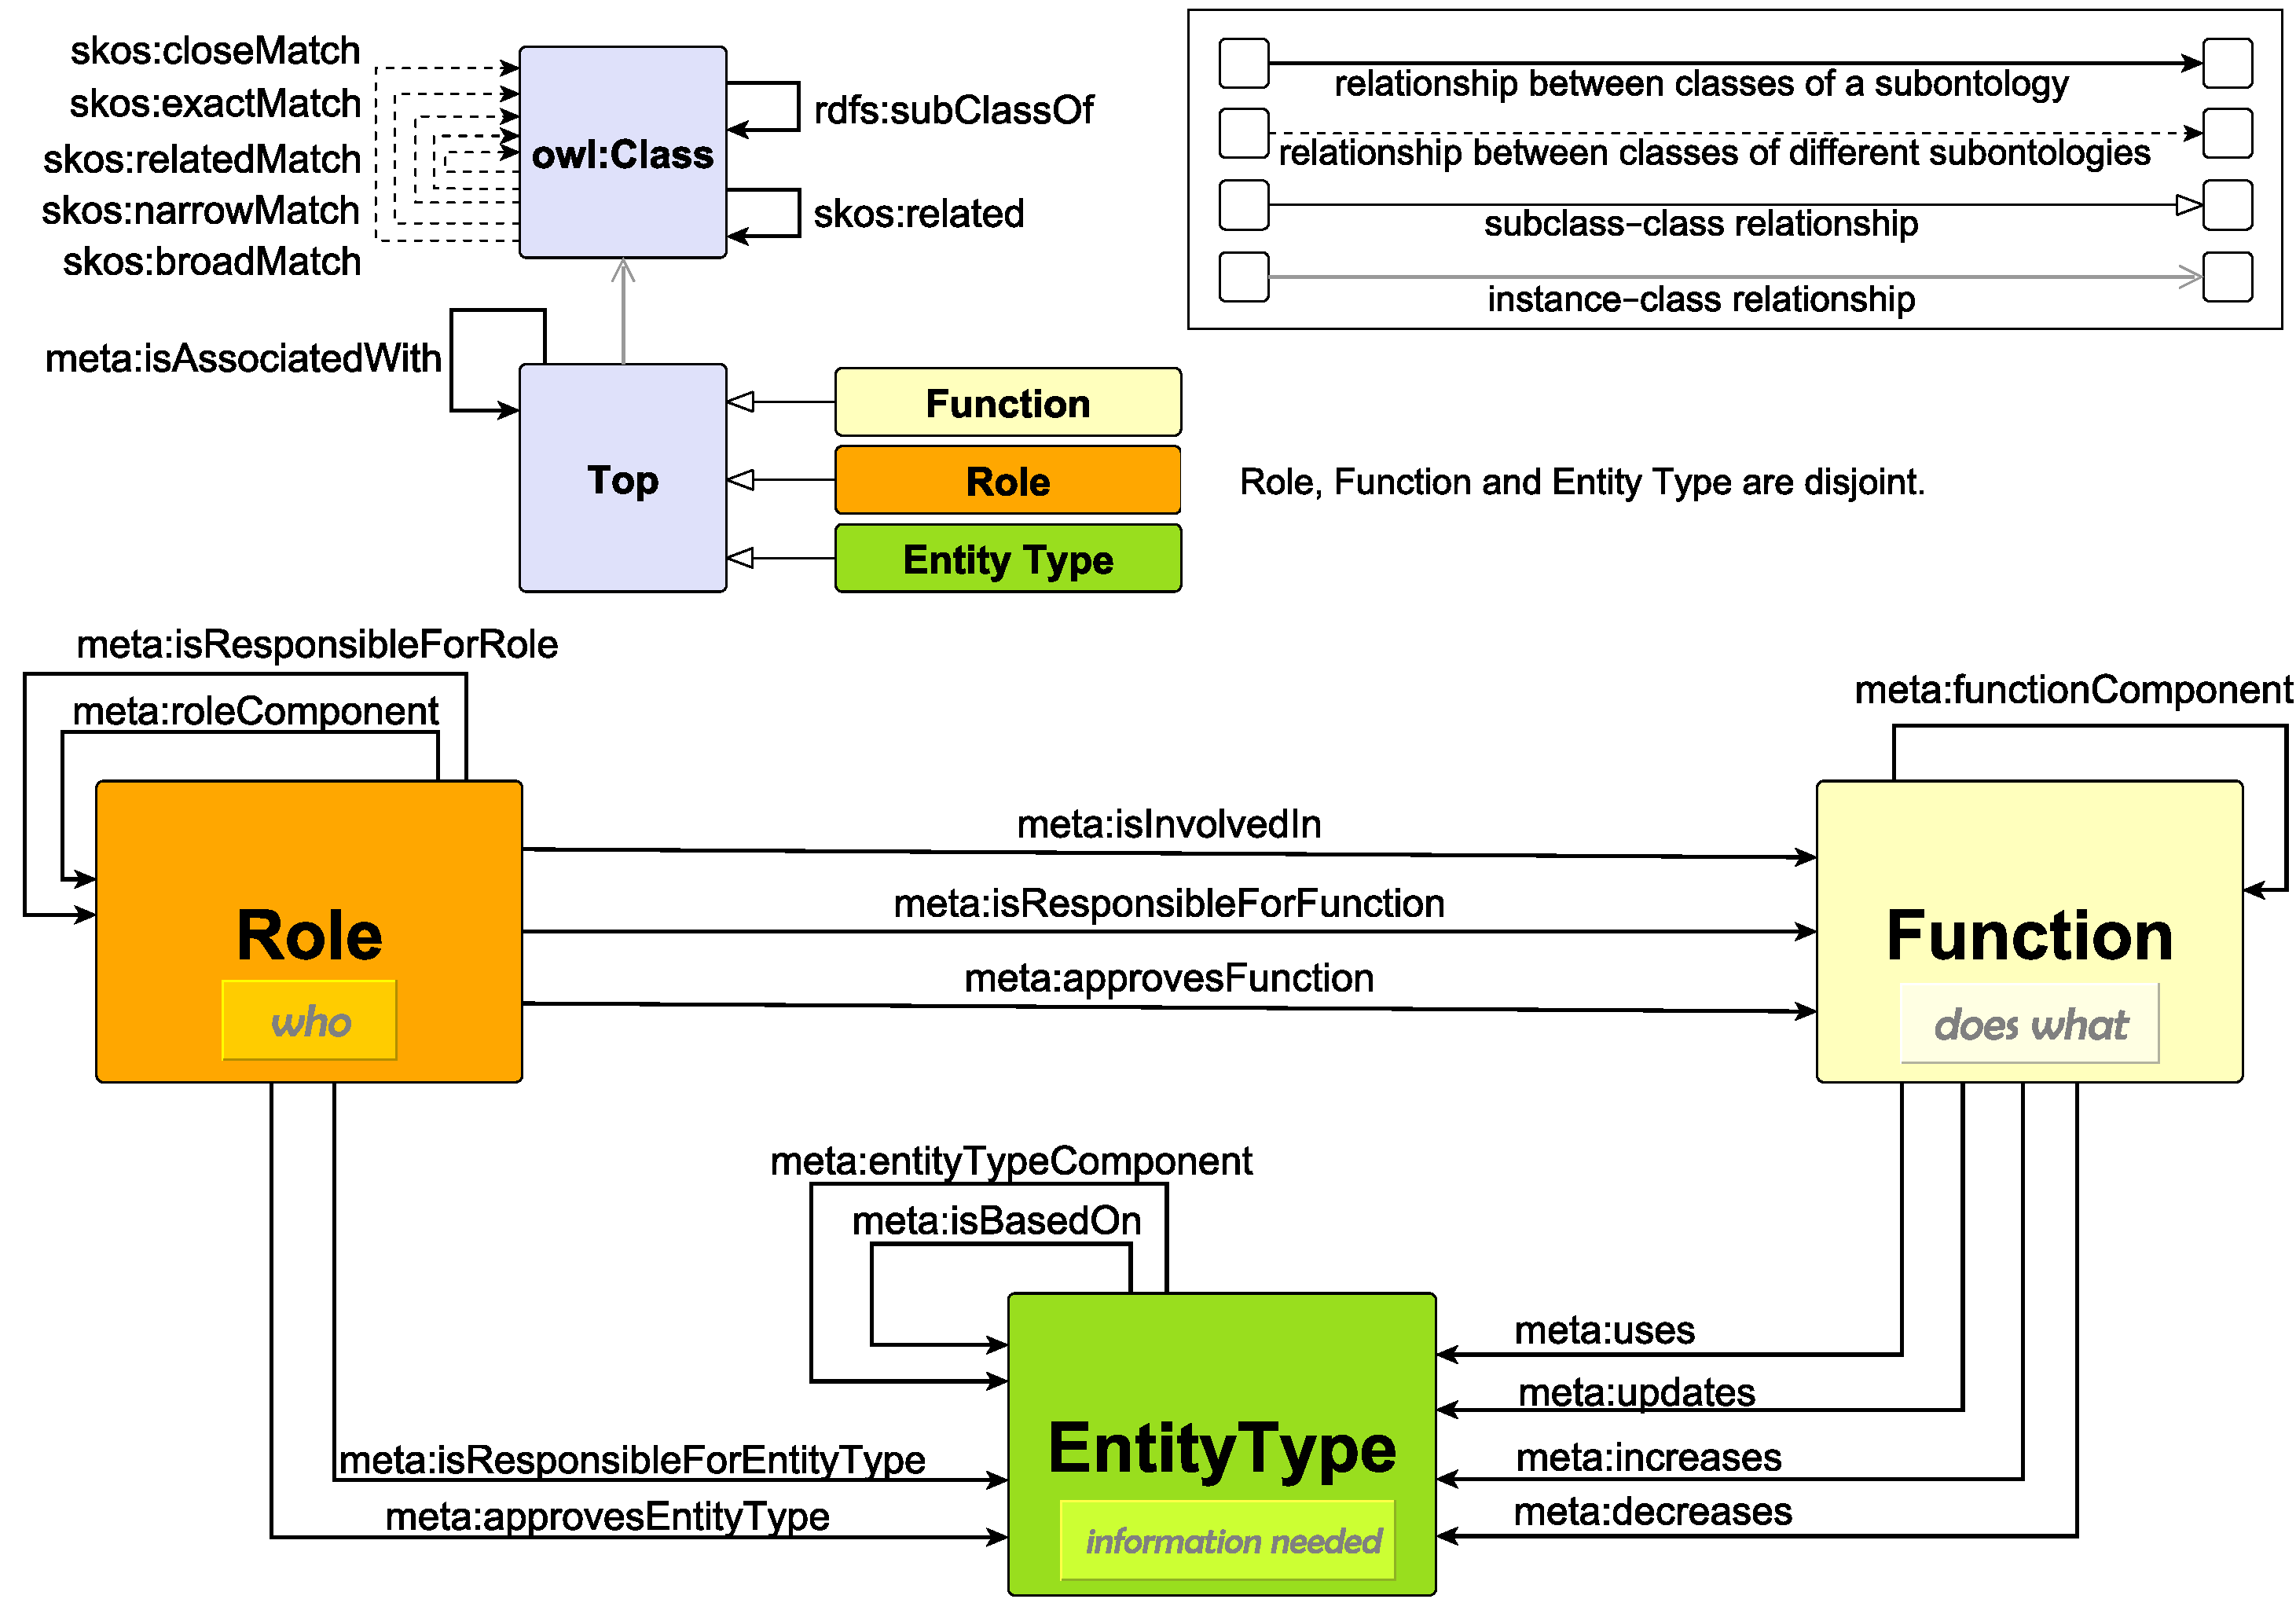
\includegraphics[width=\linewidth]{metamodel9s.pdf}
    \caption{The Meta Model of the SNIK Ontology~\cite{snikposter}. SNIK contains 4118 classes, including 226 roles, 1085 functions and 2636 entity types as of 2021-02-21.}\label{fig:metamodel}
\end{figure}

\begin{table}[h]
\centering
\caption{Namespaces.}
\label{tab:namespaces}
\begin{tabularx}{\linewidth}{|l|X|l|l|}
%\toprule
\hline
\textbf{Prefix}	&\textbf{Ontology}				&\textbf{Source}		&\textbf{Color}\\
%\midrule
meta	&\url{http://www.snik.eu/ontology/meta}		&Meta Model			&red\\ \hline
bb		&\url{http://www.snik.eu/ontology/bb}		&Textbook~\cite{bb}	&blue\\\hline
ob		&\url{http://www.snik.eu/ontology/ob}		&Textbook~\cite{ob}	&orange\\\hline
he		&\url{http://www.snik.eu/ontology/he}		&Textbook~\cite{he}	&green\\\hline
ciox	&\url{http://www.snik.eu/ontology/ciox}		&CIO Interview		&cyan\\\hline
%\url{http://www.snik.eu/ontology/it4it}		&Standard~\cite{it4it}\\\hline
%k\bottomrule
\end{tabularx}
\end{table}

\subsection*{Design Goals and Requirements}
Our main goal is to visualize knowledge extracted from text books to users that may not have any Semantic Web experience.
The time and cognitive load of the users required to install, learn and operate the application should be as low as possible, so that they can focus on the data at hand and experience a benefit compared to only reading the textbook, such as when studying for an exam.
A web application is easiest to set up for the user, as it is operating system agnostic and does not need to be installed.
%\todo{Vorschlag von Michelle: Verwendung in der Lehre setzt intuitive/leicht erlernbare Benutzung des Graphen voraus um zu vermeiden wertvolle Vorlesungszeit an ein Tutorial zu verlieren --> Bekannet Tastaturshortcuts, Drag and Drop, übersichtliches }




\section*{Implementation and Setup}
As none of the investigated existing approaches support all our use cases and design goals and provide adequate performance on more than 4000 nodes, we implemented SNIK Graph as a web application using JavaScript (EcmaScript 2015) based on the graph visualization library Cytoscape.js~\cite{cytoscape}.
SNIK Graph is freely available as open source software\footnote{\url{https://github.com/imise/snik-cytoscape.js}}.
As a client-side tool\footnotemark{}, SNIK Graph can be adapted for other knowledge bases and ontologies and published on any HTML web server by cloning the repository, installing the NPM dependencies and adapting the configuration file settings including the SPARQL endpoint URL.
\footnotetext{Aside from a SPARQL endpoint.}%
An installation containing SNIK is published at \url{https://www.snik.eu/graph}.

\section*{Features}
 

\subsection*{Tabs and Containers}
\begin{figure}[h]
    \centering
    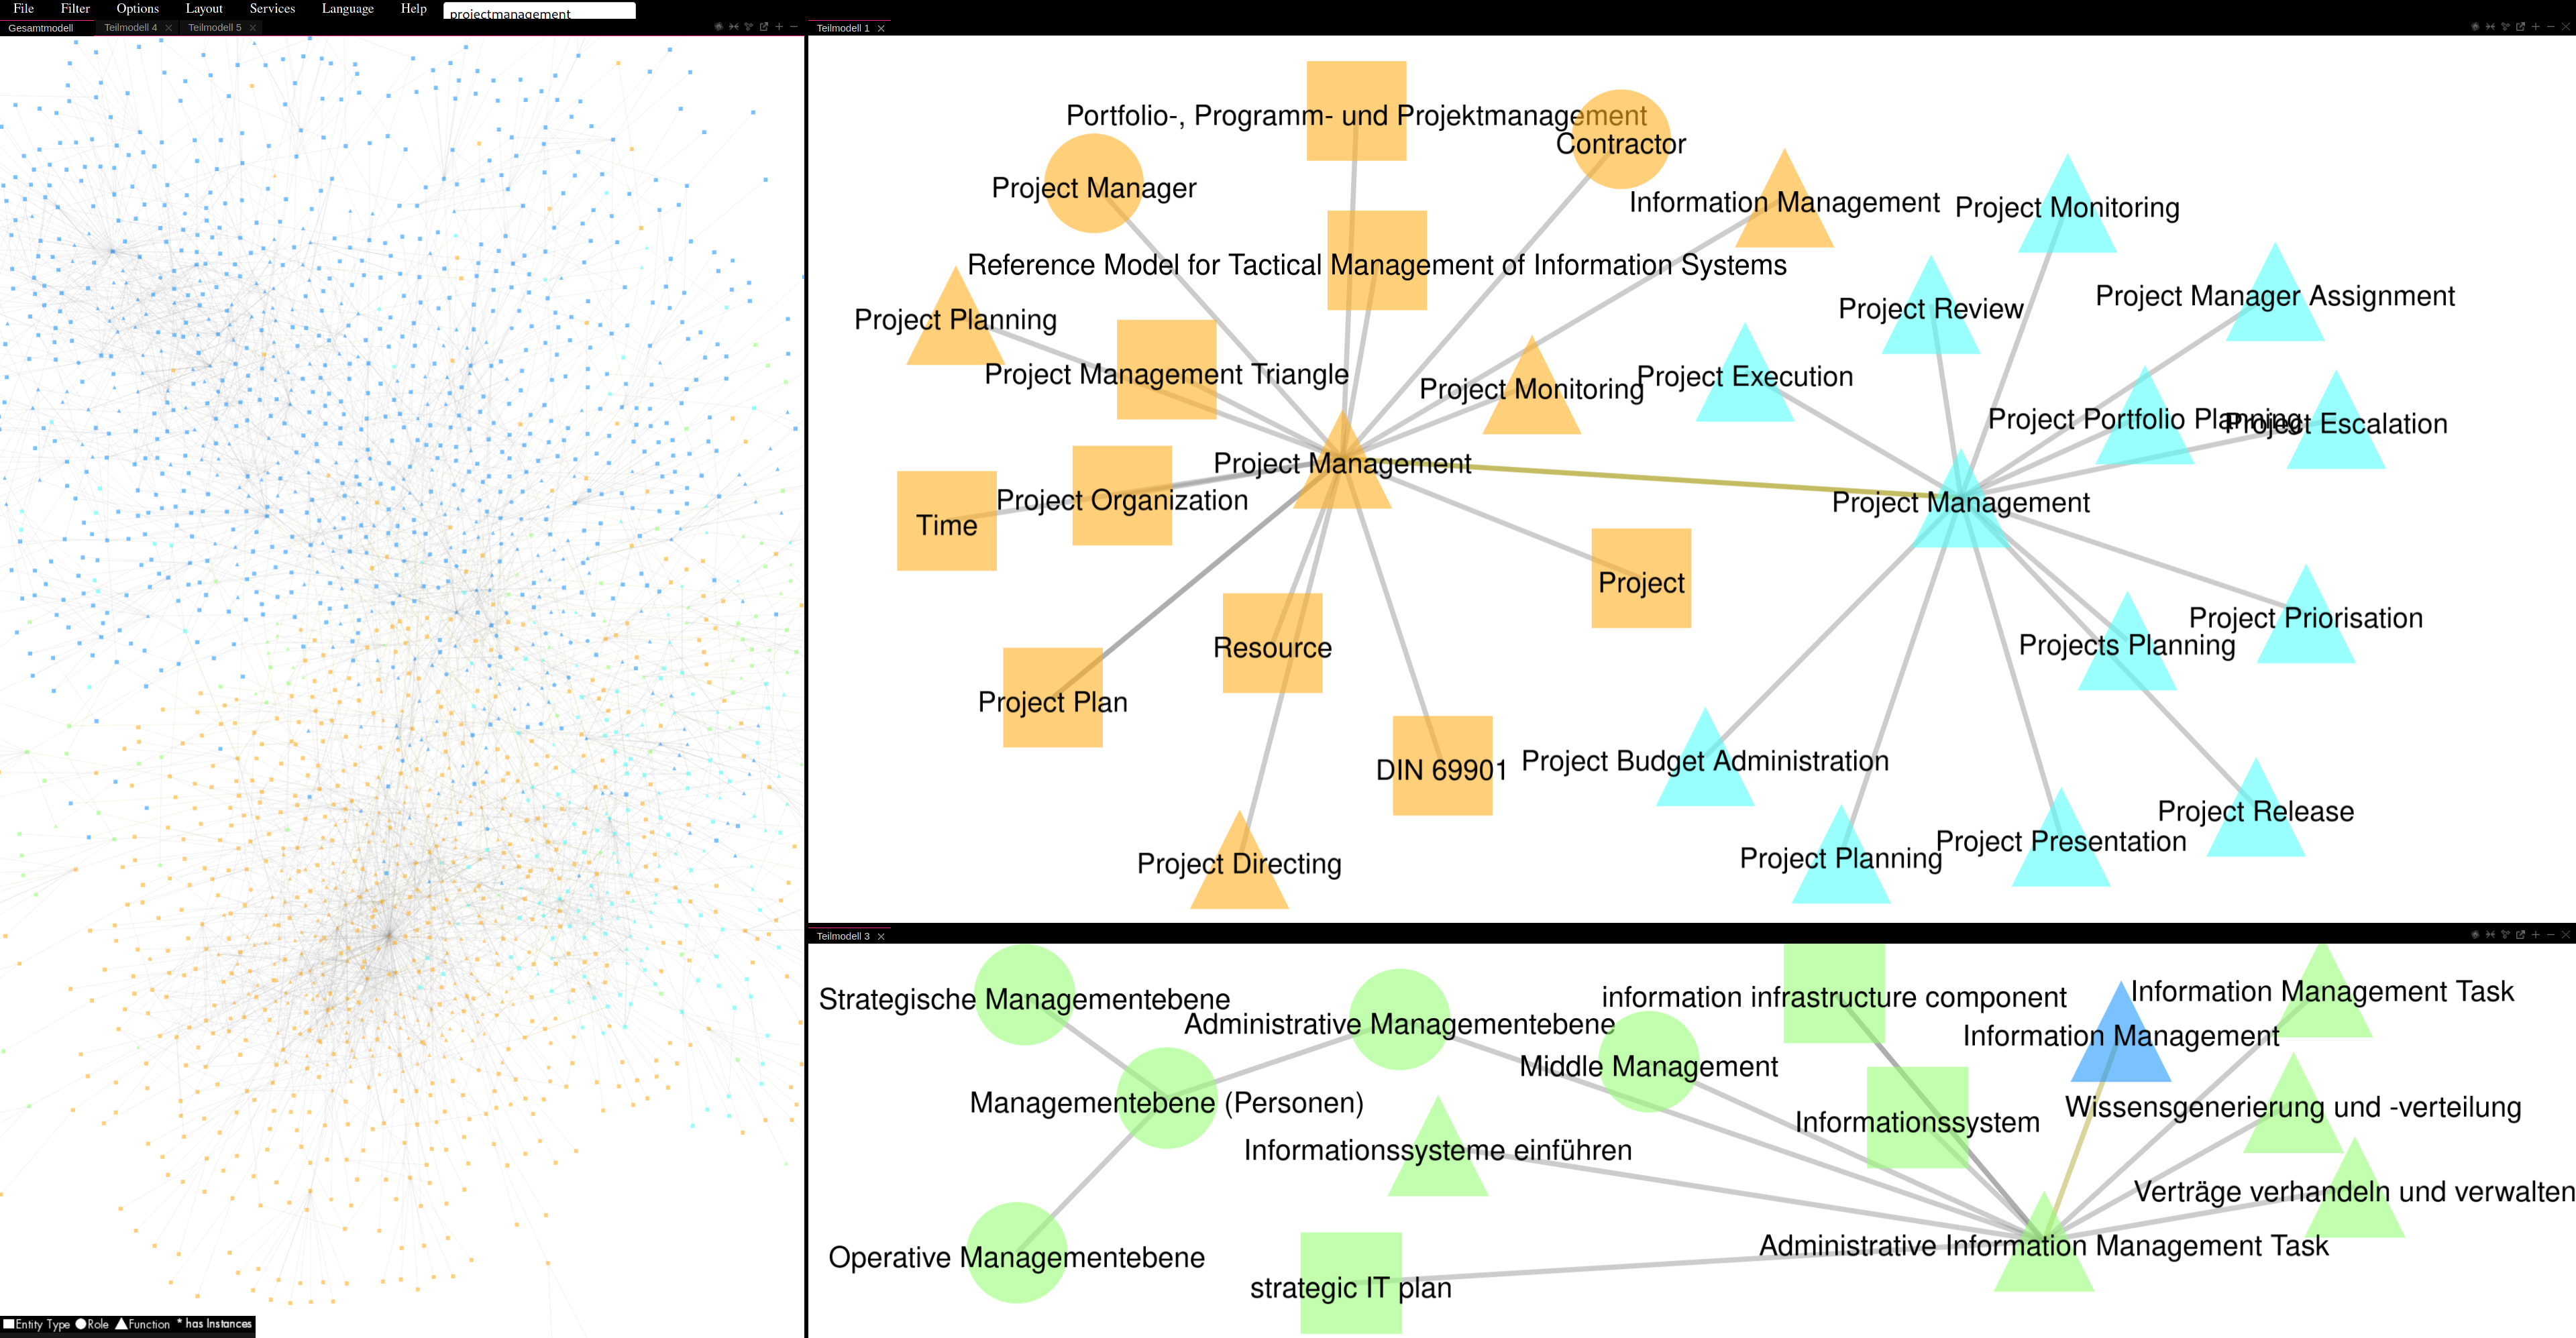
\includegraphics[width=\linewidth]{tabs.png}
    \caption{A session containing the default view and freely partitioned subgraphs containers.}
	\label{fig:tabs}
\end{figure}
\vspace{-3pt}
%For this subgraphs of the ontology have to be extracted and organized.
%A feature of SNIK Graph, tabs, allows multi-instance usage.
%One major issue in working with SNIK Graph was the missing ability of organizing teaching scenarios.
To organize teaching scenarios, independent SNIK Graph instances are loaded into containers\footnotemark{} that can be organized around the browser window.
\footnotetext{Implemented using the JavaScript GoldenLayout framework (\url{https://golden-layout.com/}).} 
These containers can either be accessed as tabs or freely partitioned see \cref{fig:tabs}.
The content and of the all containers can be saved and loaded as a session to continue developing a teaching scenario at a later point.

%This feature allows better workflows in preparation and presentation of teaching scenarios.
%We use JSON formatted files for export and import.

\subsection*{Compound Layout}
\begin{figure}[h]
    \centering
    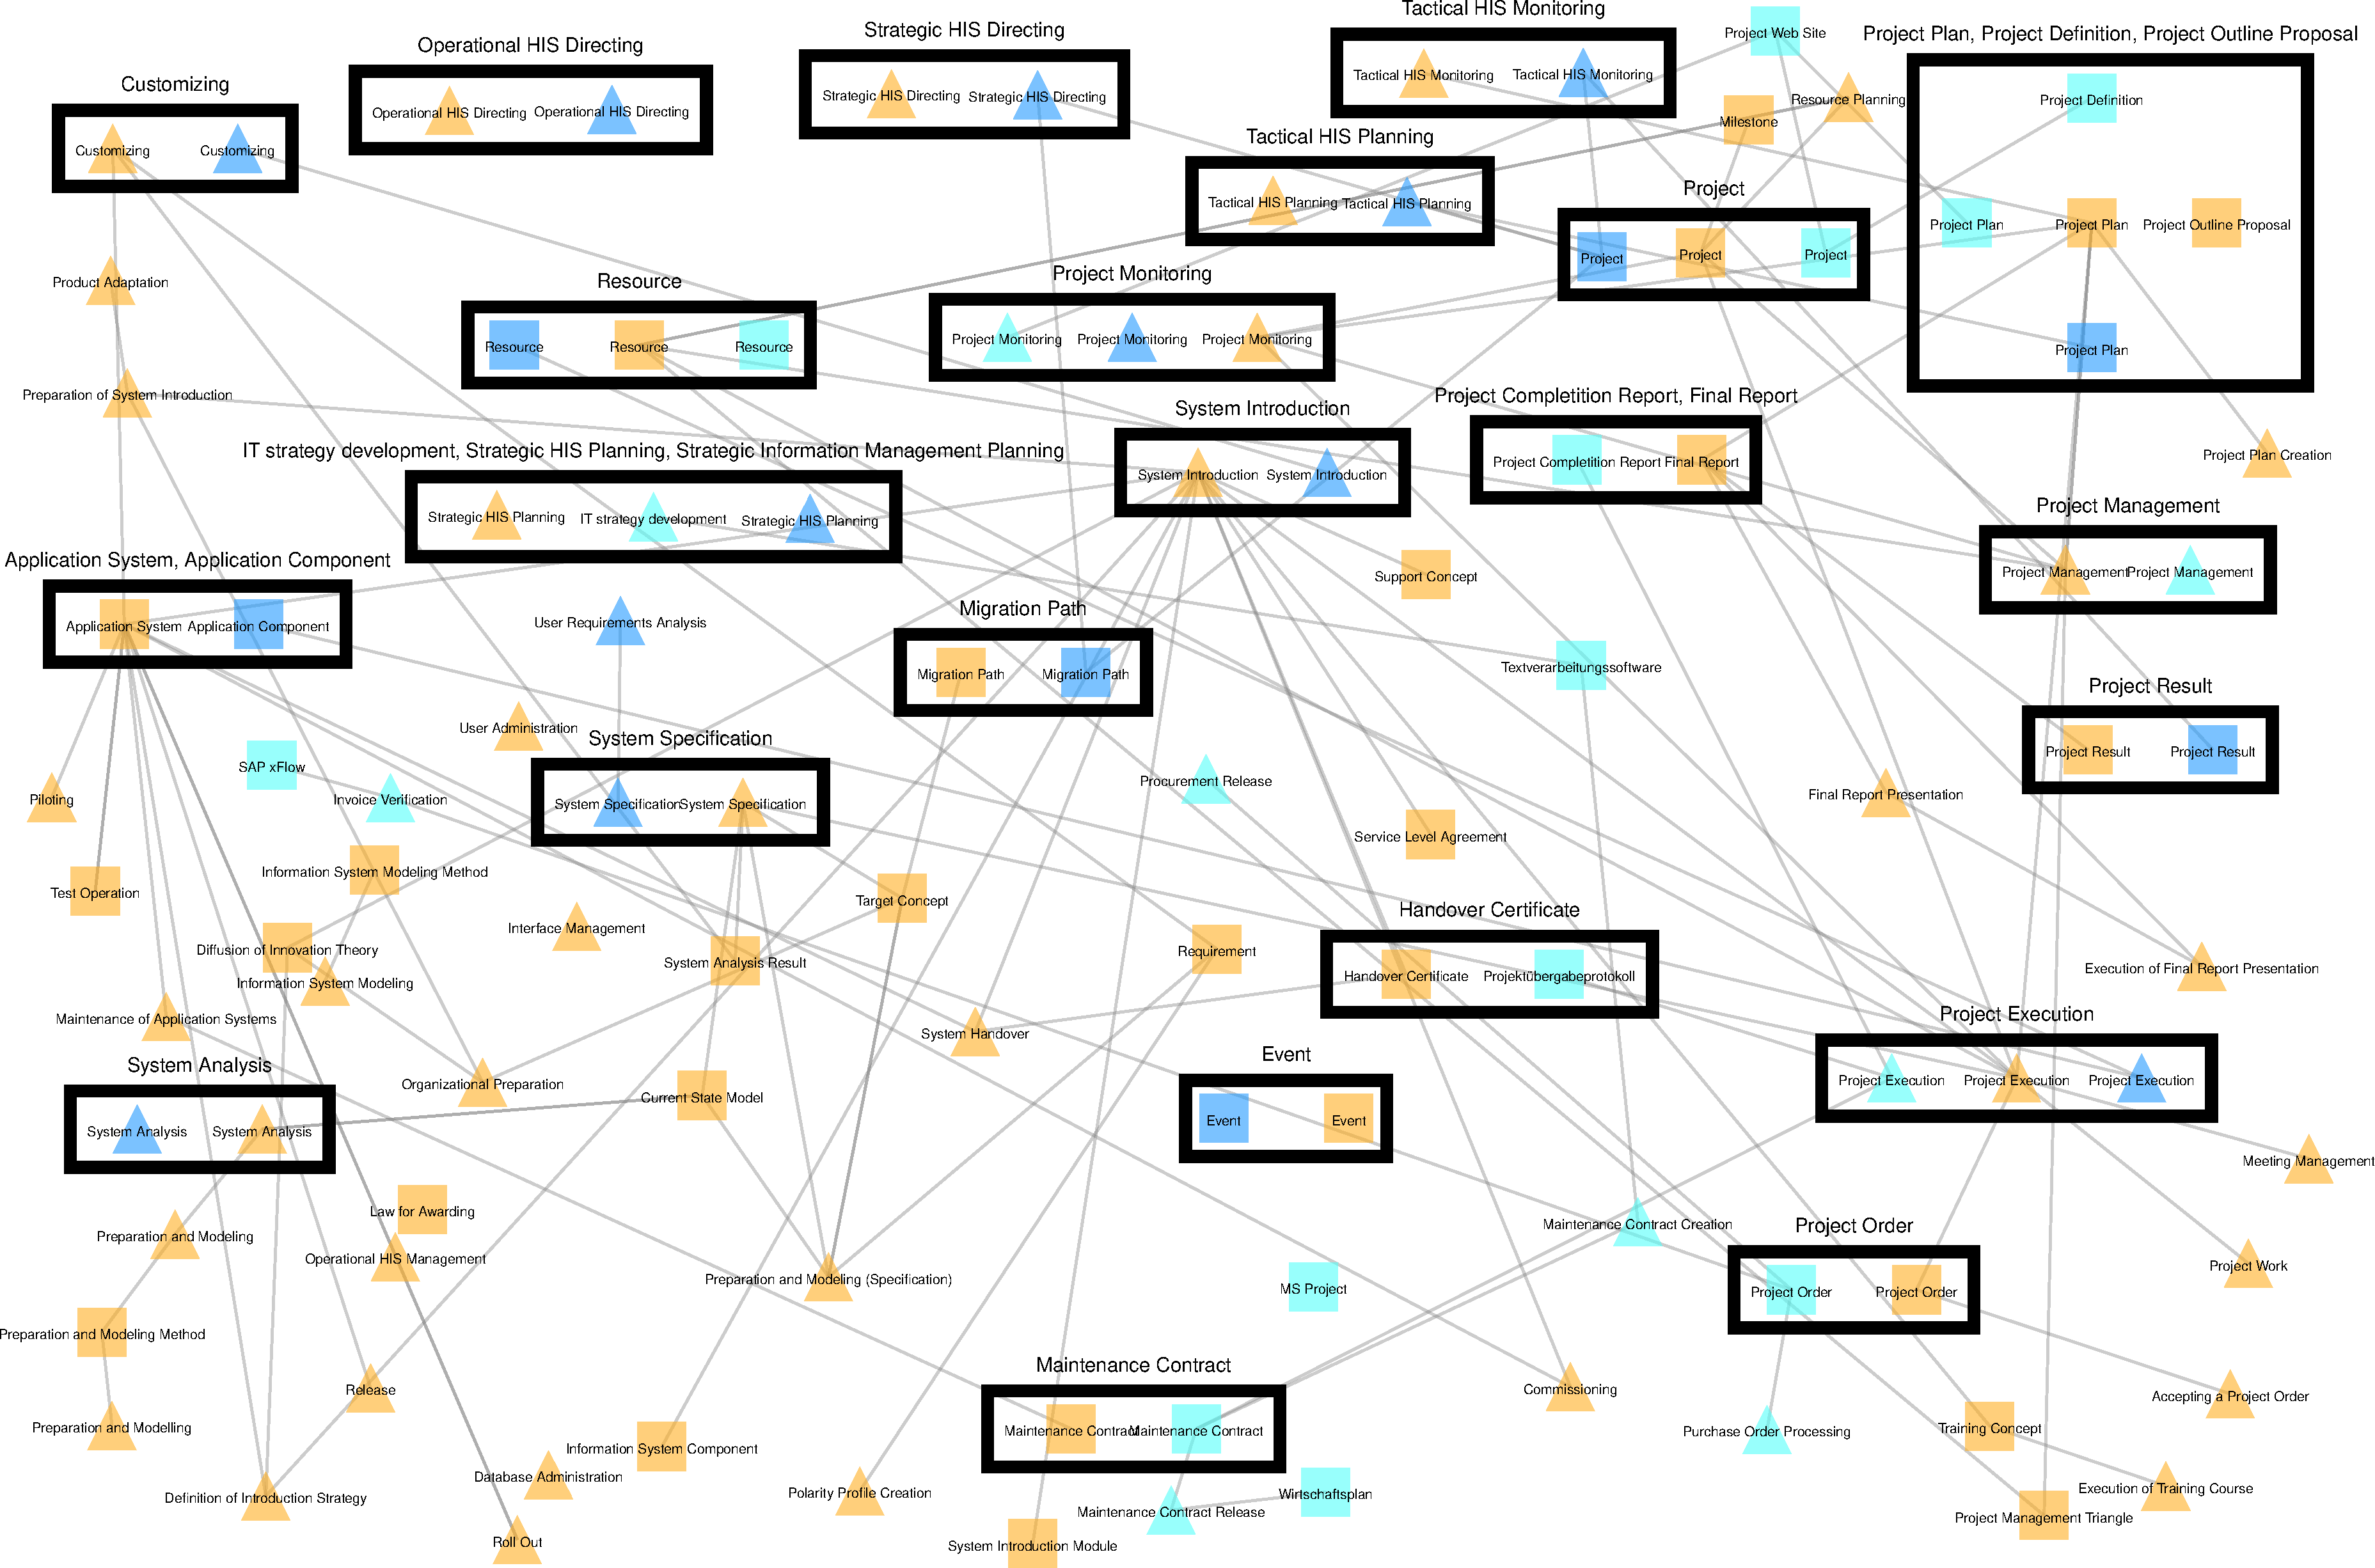
\includegraphics[width=\linewidth]{combine.pdf}
    \caption{Grouping of equivalent concepts from different sources in SNIK Graph (color coded).}% using the \enquote{combine matches} option.}
	\label{fig:combine}
\end{figure}
\vspace{-3pt}
%\noindent For citations of references, we prefer the use of square brackets and consecutive numbers, e.g. as shown by Author et al. [2], [3, pp. 5–10], as mentioned earlier [1], [3], [9]. The following bibliography provides the basic formats as a reference list with entries for journal articles [1], book chapter [2], as well as a URL [5]. For further guidance please refer to the \href{https://ieeeauthorcenter.ieee.org/wp-content/uploads/IEEE-Reference-Guide.pdf}{IEEE-Reference-Guide}.

Users can group interlinked nodes together and either display them side by side or on top of each other, see \cref{fig:combine}.
As SNIK consists of more than 4000 classes, viewing large parts of it at once does not convey much information.%, see \cref{fig:much}.
To alleviate this, SNIK offers multiple exploration methods described in the following.
%\begin{figure}[h!]
%    \centering
%    \includegraphics[width=\linewidth]{much.pdf}
%    \caption{Excerpt of SNIK using the default force directed layout.}\label{fig:much}
%\end{figure}

\subsection*{Role Use}
\iffalse
\todo{konrad an alle: was mache ich mit der sparql query? rausschmeissen, drin lassen oder umbauen? TP: drinlassen, aber direkt ans Bild hängen.. Sowas wie aus der Query folgt dieses Bild. Ich finde sowas sollte schon rein ins Paper}
\begin{figure}[h]
\begin{lstlisting}
SELECT DISTINCT ?inner ?middle ?outer ?outerx {
 <role> (rdfs:subClassOf|skos:closeMatch|^skos:closeMatch)* ?inner.
 ?inner meta:subTopClass meta:Role.
 OPTIONAL {
  ?inner ?p ?middle.
  ?middle meta:subTopClass meta:Function.
  OPTIONAL {
   ?middle ?q ?outer.
   ?outer meta:subTopClass meta:EntityType.
   OPTIONAL {?outer (skos:closeMatch|^skos:closeMatch|^rdfs:subClassOf)+ ?outerx.}
}}}
\end{lstlisting}
\caption{SPARQL query to generate the \emph{role use} visualization.}
\label{lst:roleuse}
\end{figure}
\vspace{-3pt}
\fi
A frequent question is, what a given role does and which information is needed for those functions represented by the entity types connected to those functions.
This question is visually answered by the \enquote{role use} feature, which arranges roles, functions and entity types in concentric circles, see \Cref{fig:classuse}:

\begin{enumerate}[align=left, labelwidth=1ex]
\item The first ring consists of the given role and all roles that are connected by a path of \aurl{rdfs}{subClassOf} and \aurl{skos}{closeMatch} edges.
\item The function ring consists of all functions adjacent to roles in the inner ring.
\item The third ring consists of all entity types adjacent to functions in the middle ring.
\item The final ring consists of all entity types that are connected to entity types from the third ring by a path of \aurl{skos}{closeMatch} and reverse \aurl{rdfs}{subClassOf} edges.
\end{enumerate}
\begin{figure}[h!]
    \centering
    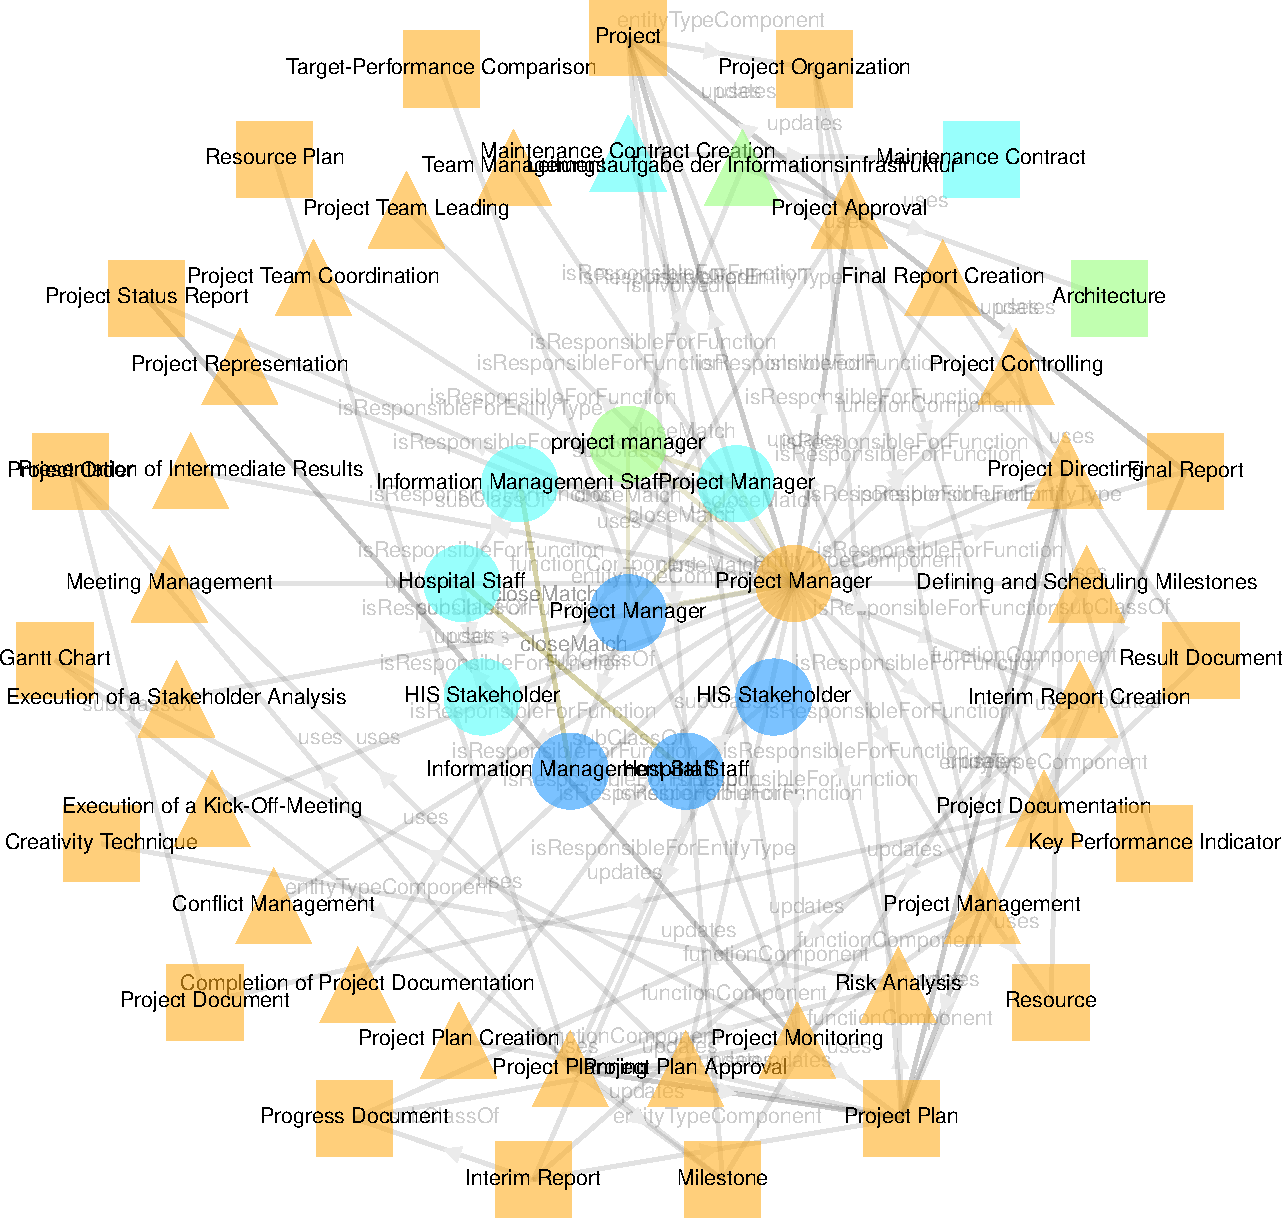
\includegraphics[width=0.6\linewidth]{class-use-project-manager.pdf}
    \caption{\emph{Role Use} of \aurl{bb}{ProjectManager}. Outermost layer ommitted due to space limitiations.}\label{fig:classuse}
\end{figure}

%\section*{Approach}
%Due to its large size, visualizing all of SNIK at once  overplotting.
%At the core of SNIK Graph is incremental exploration, which starts at one or more nodes and gradually expands them to related ones.

\subsection*{Search}
\begin{figure}[h!]
    \centering
    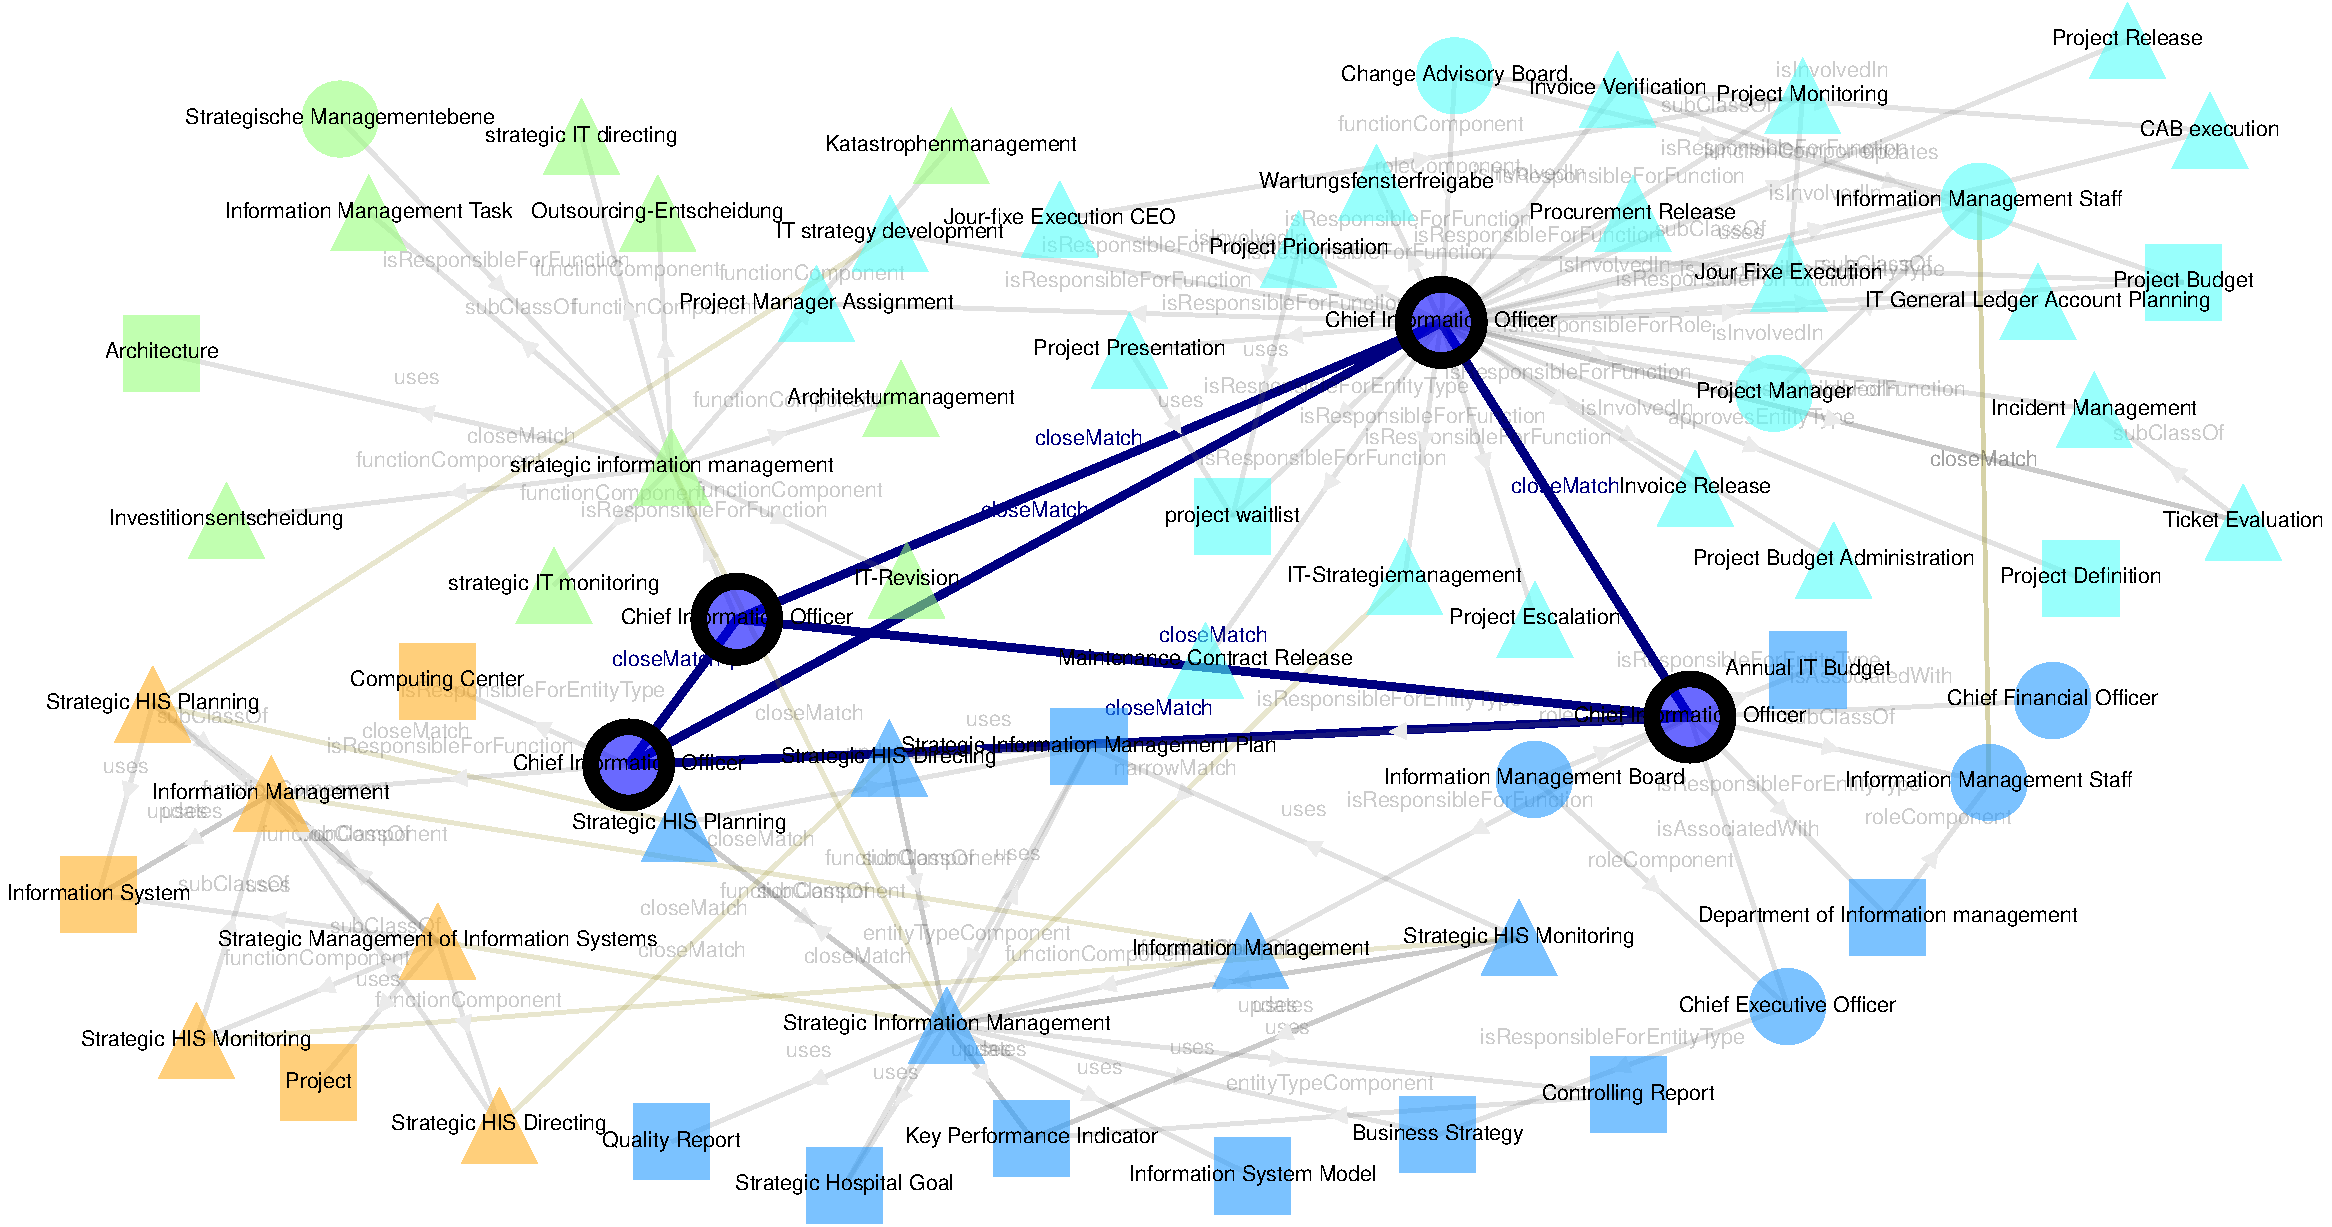
\includegraphics[width=\linewidth]{search.pdf}
    \caption{Visual search results for \enquote{Chief Information Officer} in a part of SNIK.}\label{fig:search}
\end{figure}

Due to the large amount of resources, exploration often begins with a search.
The search index is populated from the target SPARQL endpoint and is implemented using the Fuse.js library that is based on the Baeza-Yates--Gonnet algorithm~\cite{textsearching}.
Fuse.js\footnotemark{} is a light-weight, purely client side JavaScript library and presents an alternative to backend-driven indexes like Lucene.%
\footnotetext{\url{https://fusejs.io/}, \url{https://github.com/krisk/Fuse}}
This enables fast fuzzy search on any dataset loaded via SPARQL endpoint but requires waiting for index initialization on the first search of each user session.
Search results presented to the user are color coded in three categories: visible (green), invisible (yellow)%
\footnote{The resource is either \emph{filtered} or \emph{hidden}.}% \cref{sec:visibility}
 and not loaded (red)%
\footnote{The resource is included in the search index built from the SPARQL endpoint but either deleted in the graph or not loaded in the first place, such as due to configuration.}.
Each search entry of a class contains the label values of \aurl{rdfs}{label} (long form) and \aurl{skos}{altLabel} (short and alternative forms) with a weight of 0.7.
Textbook definitions are included with a weight of 0.3.
Labels of resources connected via \aurl{skos}{closeMatch} interlinks in either direction are included as well, because those resources are defined as semantically close, so we assume their labels are synonyms.
Fuzzy matching is enabled with a threshold of \num{0.25}.
The resource \aurl{bb}{ChiefInformationOfficer} can thus be found by entering either \enquote{CIO} (alternative label), \enquote{vice president} (part of the definition) or \enquote{Leiter des Rechenzentrums} (German alternative label of \aurl{ob}{ChiefInformationOfficer}).
Search results are then selected in the graph, see~\cref{fig:search}, which allows further exploration by chaining the path and neighbourhood operations described in following.

\subsection*{Shortest Paths}
\begin{figure}[h!]
    \centering
    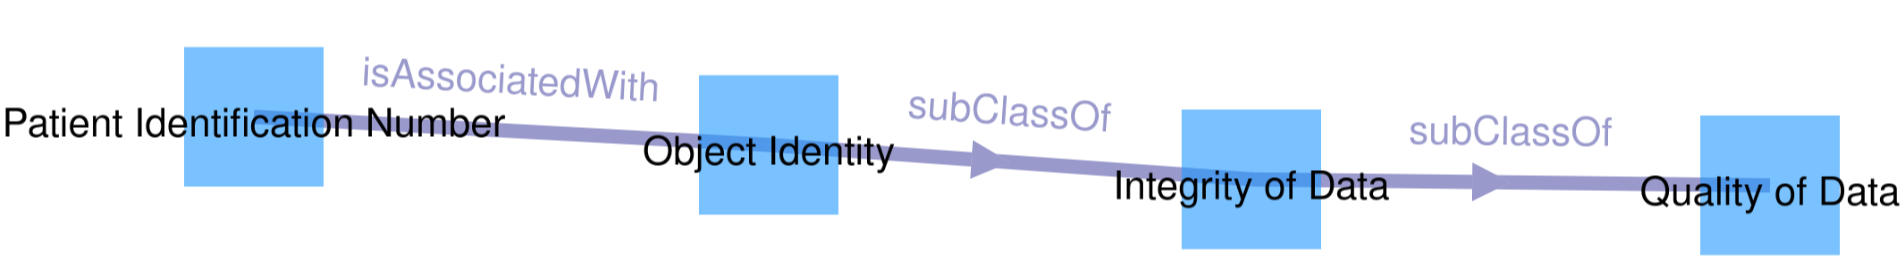
\includegraphics[width=\linewidth]{path.png}
    \caption{The shortest non-trivial path between \aurl{bb}{PatientIdentificationNumber} and \aurl{bb}{QualityOfData} in SNIK Graph.}
	\label{fig:path}
\end{figure}
\vspace{-3pt}
The shortest path is the most basic method of visualizing the relationship between two resources, see \cref{fig:path}.
We treat SNIK as an undirected graph for the calculation because the direction is often arbitrary.
Roles can be nested using \aurl{meta}{roleComponent} (\emph{has part}), which could have just as well been modelled as a \emph{part of} relation with reversed subject and object.
Another reason is that a set of resources that forms a graph connected by some symmetric property implies a complete subgraph, which negatively effects speed, memory and visibility of SNIK Graph.
For this reason, \aurl{skos}{closeMatch} and other symmetrical properties are often only sparsely modelled, and the other triples are implied.
As SPARQL endpoints, such as Virtuoso SPARQL employed by SNIK, do not perform reasoning to infer such implied triples such as those generated by symmetric properties, this would prevent the shortest path from including resources where only the opposite direction is explicitly modelled.%
\begin{figure}[h]
    \centering
    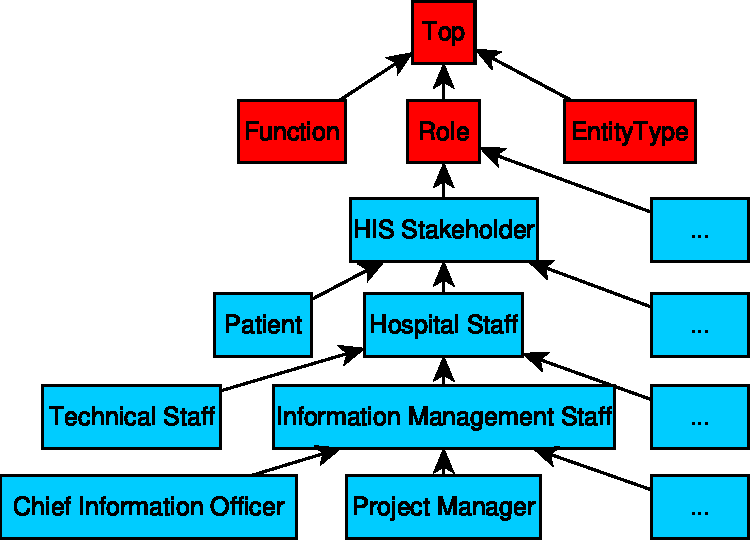
\includegraphics[width=0.5\linewidth]{hierarchy.pdf}
    \caption{Excerpt of the SNIK class hierarchy. Source: \cite{snikposter}.}
	\label{fig:hierarchy}
\end{figure}
\vspace{-3pt}
We also don't explicitly store triples inferred by transitive properties such as \aurl{rdfs}{subClassOf}, which prevents paths involving such properties from being squashed, such as the path between \emph{Project Manager} and \emph{HIS Stakeholder} in \cref{fig:hierarchy}.


%We ignore the direction of edges because, that is, which resource is the subject and the object 
The largest problem of shortest paths is however, that they are not necessarily informative to the user. 
For example, any two roles, such as \aurl{bb}{ChiefInformationOfficer} and \aurl{bb}{ChiefExecutiveOfficer}, are connected by a path of length 2 as they are all subclasses of \aurl{meta}{Role}, which the user already knows given the triangular shapes representing roles in SNIK Graph.
To exclude such trivial paths,  the meta model is not shown by default.
Furthermore, filtering, such as by knowledge source or type of relation or resource, allows further tuning of the resources that are shown and eliglible for paths.
%Further research into informative paths has been done in two bachelor theses~\cite{}.
An general approach to solve the problem of informative shortest paths is \emph{weighted shortest paths for RDF graphs (WiSP)}~\cite{wisp}.
Future work includes adopting this approach to SNIK Graph and evaluating it with its users.
Another approach is to show all short paths under a given length and let the user remove unwanted ones manually, as employed by \emph{Relfinder}~\cite{relfinder}.

\subsection*{Neighbourhood Operations}
Exploration using neighbours, that is the successive uncovering of nodes adjacent to a starting node given by a user, is a common feature of tools such as \cite{lodlive} and \cite{vizlod}.%
\subsection*{Star}
The directed and undirected star operations show nodes connected to selected nodes via all paths that contain at most one property other than \aurl{skos}{closeMatch}.
The \emph{circle star} also rearranges the nodes using the force-directed layout locally on the currently visible subgraph.
\Cref{fig:star} shows a mind map of strategic information management, created by an undirected star, which can be used by a teacher to prepare a lecture about the topic.
\begin{figure}[h!]
    \centering
    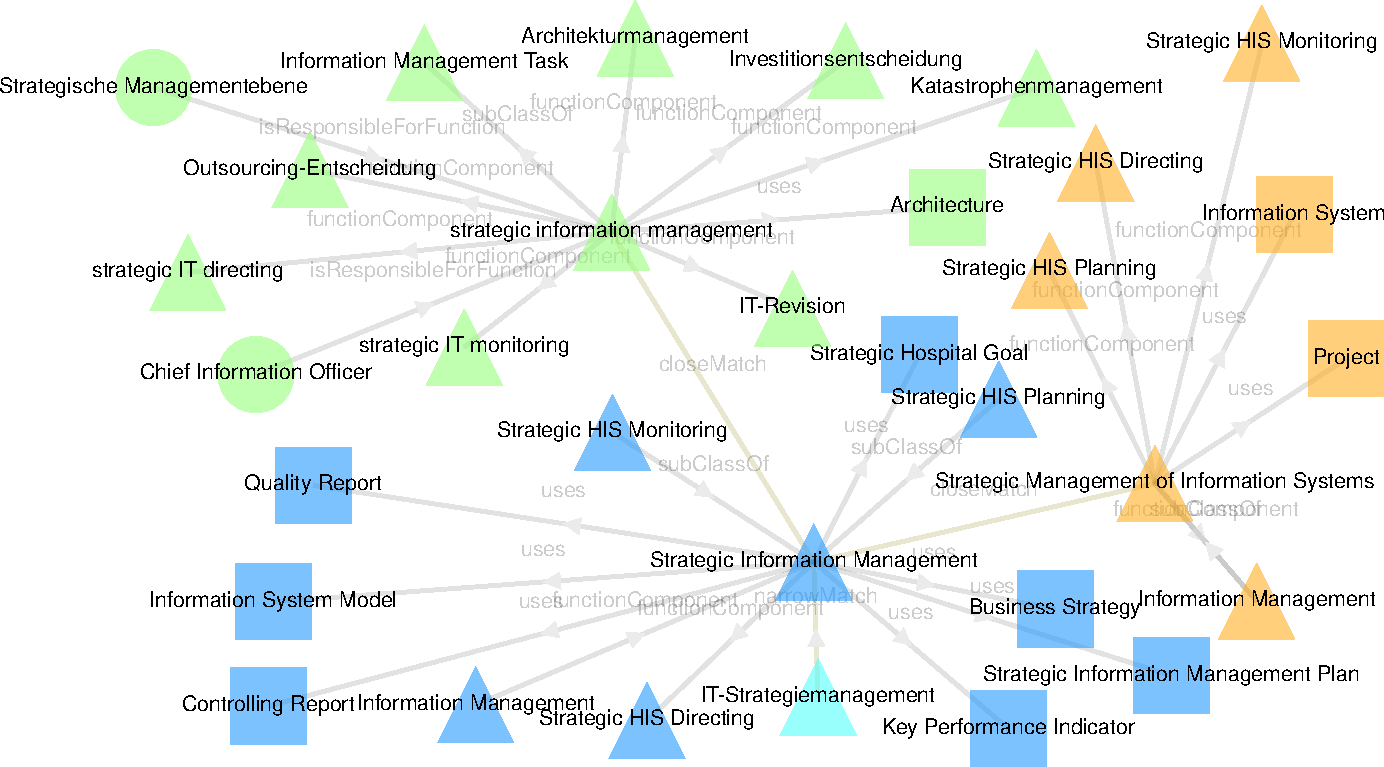
\includegraphics[width=0.9\linewidth]{strategic-im.pdf}
    \caption{Undirected \emph{Star} of \aurl{bb}{StrategicInformationManagement}.}
	\label{fig:star}
\end{figure}
\vspace{-3pt}

%\todo{Konrad: Nimm den Star um "ob/ProjectManagement".} % ist inkludiert in \cref{fig:tabs}, refer?
The concept \emph{project management} both exists in a textbook~\cite{ob} and in the knowledge about information management in a German university hospital.
Grouping both concepts with the help of the star function the user detects that the terms have a different meaning according to their neighboorhood terms.
Whereas the text book deals with the management of single projects, in the CIO's world \enquote{project management} means managing multiple projects, as shown in the lower right container in \cref{fig:tabs}.


\subsection*{Mixed Operations}
\subsubsection*{Spiderworm}
A \emph{spiderworm} is a path from node \emph{A} to node \emph{B} combined with a \emph{star} of \emph{B}.
\Cref{fig:spiderworm} shows how we use a spiderworm to teach a student how the new concept \enquote{quality of data} is connected the the already introduced concept \enquote{patient identification number.}

\begin{figure}[h!]
    \centering
    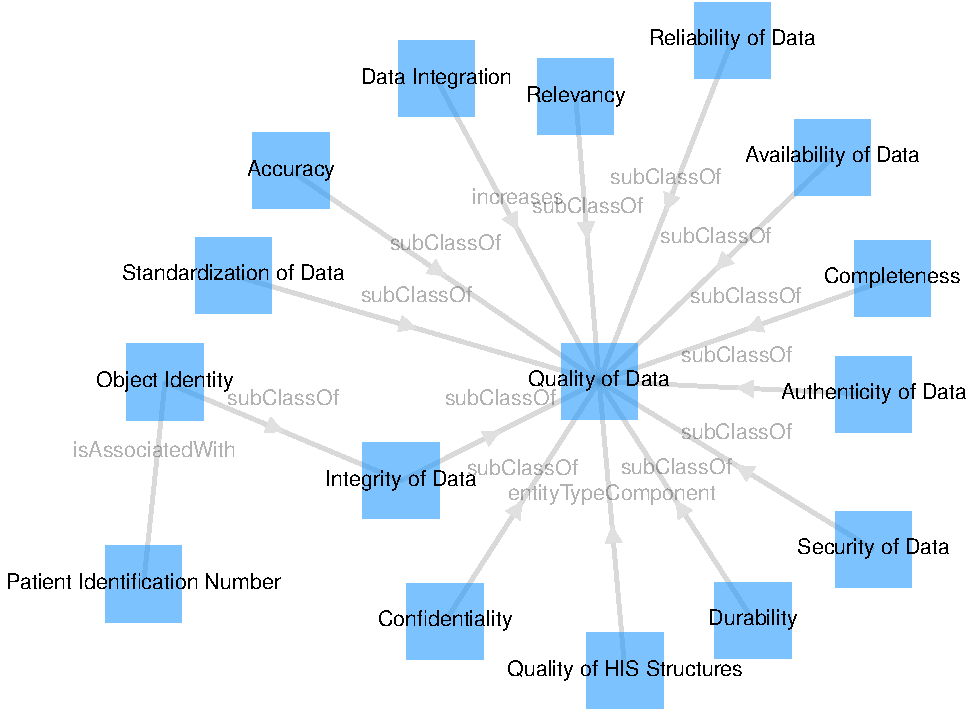
\includegraphics[width=0.5\linewidth]{spiderworm.pdf}
    \caption{\emph{Spiderworm} from \aurl{bb}{PatientIdentificationNumber} to \aurl{bb}{QualityOfData}~\cite{snikgraphposter}.}
	\label{fig:spiderworm}
\end{figure}
\vspace{-3pt}

\section*{Conclusions and Future Work}
With SNIK Graph, we implement an adaptable open-source client-side graph-based Linked Data visualization that supports both A-Boxes and T-Boxes covering 11 of the 15 use cases presented in~\cite{linkeddatavisualization}.
We publish an installation visualizing the SNIK ontology and use it for teaching and self-learning of HIS management.
SNIK Graph is easy to setup and can be configured to visualize other knowledge bases and ontologies.  
Our main focus on improvement is the performance, which is mostly adequate on more than 4000 nodes, but suffers in two key areas:
% A problem is that related approaches are not available as open source ...
% this hinders analysis and slows progress, as effort is not shared and ...
%\section*{Evaluation}
%SNIK Graph is evaluated on the SNIK dataset, which contains textbook knowledge about the management of hospital information systems.

%Different presentation forms are suitable for different use cases and data sets.
% RDF browsers are well suited for ...

%\subsection*{Future Work}
%\subsection*{Performance}
%On graphs of several thousand nodes, 

%(1) Performing a force directed 
\subsection*{Force-Directed Layouts}
Due to its client-side design, the initial\footnotemark{} single-threaded force-directed layout generation of the full graph takes around 15 seconds on an Intel i9-10900k and significantly longer on older machines.
\footnotetext{For following uses, the layout is cached in the local storage of the browser.}%
As CPUs with 6 to 16 cores become the norm, the speed penalty of single-threaded code becomes enormous.
Thus, the single-thread paradigm of JavaScript seriously hinders performance of CPU-bound applications like SNIK Graph.
While web workers\footnote{\url{https://html.spec.whatwg.org/multipage/workers.html\#workers}} offer multithreading for JavaScript applications, they posess separate memory and cause large overheads for serialization and deserialization and are thus not suited for short-lived tasks like calculating a single step of a force-directed layout for parts of a given graph.
Thus, a light-weight parallellization option is needed.
The WebAssembly \enquote{threads}-proposal\footnote{\url{https://github.com/WebAssembly/proposals/issues/14}} provides such a construct, however it is only at phase 2 \enquote{Proposed Spec Text Available}, which need to be followed by the implementation in browsers and the standardization phase.
The main developer of the Cytoscape.js library showed interest in then rewriting a future version in WebAssembly.

\subsubsection*{Graph Rendering}
Due to the low performance of rendering on an HTML canvas, the frame rate can drop significantly below a fluent 60 frames per second (FPS).
While Cytoscape.js buffers already rendered parts, this mechanism suffers when moving around at medium zoom levels.
The frame rate is especially low on large resolutions such as 4k (3840x2160) and on browsers other than Google Chrome / Chromium, where the minimum frame rate drops to as low as 8 FPS on an Intel i9-10900k at 4k on Mozilla Firefox 86 and 36 FPS on Chromium 88 on Arch Linux.
We attribute the large difference between Chrome / Chromium and Firefox to the different JavaScript engines.
While SNIK Graph does not require perfectly smooth motion and wild movements are not a common usage pattern, stuttering is still frustrating to users especially on less performant CPUs and browsers other than Chrome and contrary to our goals of minimizing friction for users. 
Due to the enormous power of modern GPUs, implementing an OpenGL-based renderer for Cytoscape.js has the potential to dramatically increase render speed.
High framerates would also allow the study of nausea-free virtual reality presentation for Linked Data visualization.

% 4903 edges, 2643 nodes
%\subsection*{Mobile Devices}

%- We also tried to automatically find the most interesting path but this was not successfull as it is subjective and the depends on the goal of the user.
%(link to AB bachelor thesis if allowed)


%\noindent Tables and Figures should be centered.
%
%\begin{enumerate}[align=left, labelwidth=1ex]
%    \item Numbering may be used, too.
%    \item ...
%\end{enumerate}
%
%\noindent Equations should be centered and set on a separate line.
%\begin{equation}
%    x+y=z
%\end{equation}


\paragraph{Acknowledgements}
This work is supported by the DFG (German Research Foundation) under the Project SNIK, Grant no. 1605/7-1 and 1387/8-1.% SNIK Graph is presented in poster form at \cite{snikgraphposter}. % KH2FJ: is that needed? I think not.

\section*{References}
\printbibliography[heading=none] %Uncomment if using biblatex. This command generates the refrences section automatically.
%\bibliographystyle{plain}
%\bibliography{paper,snik,relatedwork}

\end{document}
